\capitulo{6}{Trabajos relacionados}

Se van a comentar diferentes aplicaciones con funcionalidad similar al presente proyecto y compararlas con él, cabe destacar que aunque hay similitudes, no se ha encontrado en el mercado ninguna solución con las características de framework de medición y extensibilidad a diferentes forjas que tiene el presente proyecto.

\section{\textit{Criticality-Score}}
Se trata de una aplicación de consola escrita en \textit{Python} por miembros del \textit{Open Source Security Foundation (OpenSSF)} \footnote{\textit{Open Software Security Foundation}:  \url{https://openssf.org/} - \url{https://github.com/ossf}} que tiene como objetivo valorar con una puntuación crítica a todos los proyectos \textit{open source} posibles para así ver de qué proyectos depende más la comunidad de desarrolladores de todo el mundo y poder así aumentar la seguridad de dichos proyectos.\\

Podemos encontrar la aplicación en:\\
\url{https://github.com/ossf/criticality_score}


La puntuación de criticidad de un proyecto define la influencia y la importancia de un proyecto. Es un número entre 0 (menos crítico) y 1 (más crítico). Se basa en el algoritmo de medida de la criticidad de Rob Pike  \footnote{\textit{Quantifying Criticality by Rob Pike}  \url{https://github.com/ossf/criticality_score/blob/main/Quantifying_criticality_algorithm.pdf}} que utiliza una serie de parámetros como las fechas de creación y actualización del proyecto, el número de colaboradores o el número de \textit{issues} cerradas entre otros. Una vez se tienen los parámetros obtenidos de los repositorios, se opera con ellos utilizando el algoritmo y se obtiene una puntuación (el \textit{criticality-score}.

En este proyecto se trabaja con repositorios de \textit{GitHub} y \textit{GitLab} utilizando \textit{API-token} como en el presente proyecto, sin embargo no es extensible a otras forjas de repositorios. Tampoco se tiene umbrales para los parámetros y no podemos valorar con esta herramienta si los valores obtenidos para calcular el \textit{criticality-score} son apropiados o no.


\section{\textit{Agile-Metrics}}
\textit{Agile Metrics} es un recopilador de datos de \textit{KPI} del proceso de desarrollo de software. Recopila mediciones de los productores (forjas de repositorios), crea métricas y las envía a los consumidores (procesadores de datos los datos de métricas para proporcionar un procesamiento posterior, por ejemplo, visualización. Sólo está soportado \textit{ElasticSearch}. Soporta tres productores o forja, \textit{BitBucket}, \textit{JIRA Software Server} y \textit{SonarQube}. Trabaja con diferentes métricas dependiendo de donde esté alojado el repositorio, por ejemplo con \textit{BitBucket} sólo calcula los \textit{commits} diarios por autor, proyecto o repositorio mientras que con \textit{JIRA Software Server} calcula 13 métricas entre las que podemos nombrar el ratio de \textit{bugs} o el volumen de \textit{issues}.\\

La idea tras la cual nace esta aplicación escrita en Java es muy similar a la del proyecto actual, pero está enfocado a necesidades más concretas pues no trabaja con las forjas de repositorios más comunes (GitHub y GitLab) y además no unifica las métricas calculadas si no que es dependiente de la forja con la que se trabaje en ese momento.

Podemos encontrar la aplicación en:\\
\url{https://github.com/DaGrisa/agile-metrics#consumer}



\section{\textit{Activity-API}}
Se trata de una aplicación desarrollada también en el entorno de un trabajo fin de carrera, similar en funcionalidad al proyecto actual. Está implementada como aplicación de escritorio en lenguaje Java y fue usado como inspiración en algunos aspectos de modelo para la primera versión inicial\cite{TFGPrevio} de este proyecto. \\
Se trata de una aplicación alojada en \textit{GitHub}\footnote{\url{https://github.com/dba0010/Activiti-Api}} y que se puede obtener y ejecutar pues es \textit{opensource}. Esta aplicación trabaja sólo con \textit{GitHub} pero tiene implementada una versión de un framework que permitiría la extensibilidad a otras forjas de manera similar a este proyecto.\\
\textit{Activity-API} permite evaluar un proyecto o comparar sólo dos entre ellos (una clara desventaja frente a este proyecto que permite añadir proyectos de forma ilimitada para compararlos). De forma similar a este proyecto muestra los resultados en forma de tabla y también trabaja con umbrales (definidos a partir de unas estadísticas obtenidas de un conjunto de datos obtenidos a partir de TFGs y publicado en \textit{GitHub} \footnote{\url{https://github.com/clopezno/clopezno.github.io/blob/master/agile_practices_experiment/DataSet_EvolutionSoftwareMetrics_FYP.csv}}  para valorar las métricas muestra los valores obtenidos para las métricas y si entran o no en los umbrales por colores como se puede ver en la  figura \ref{fig:M6_AA_Comparativa}

\begin{figure}[!h]
	\centering
	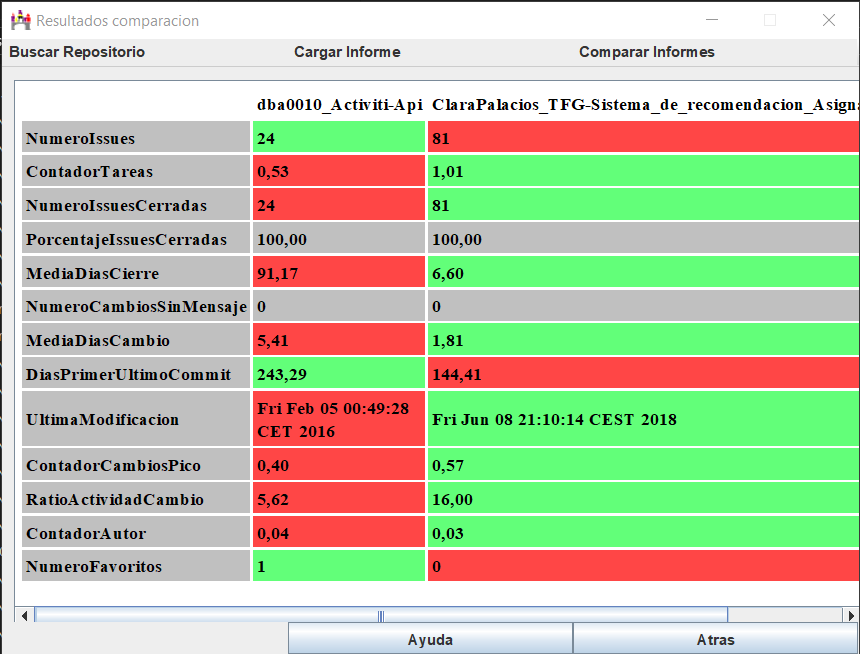
\includegraphics[width=0.65\textwidth]{M6_AA_Comparativa}
	\caption{Comparación de dos proyectos utilizando \textit{Activity-Api}}\label{fig:M6_AA_Comparativa}
\end{figure}
\FloatBarrier

Además permite la exportación de los resultados como en este proyecto aunque luego no permite importarlos.


\section{Resumen comparativo}

Podemos comparar diferentes características de las herramientas con el proyecto, comparando si son extensibles en cuanto a forjas de repositorios o métricas o no entre otras características.\\

\newpage
Como podemos ver en las tablas anteriores, el proyecto actual destaca claramente en cuanto a extensibilidad y capacidad de configuración, se pueden añadir más forjas de repositorios y nuevas métricas mientras que en el resto de herramientas es más complicado ya que están acopladas a las integraciones que tienen con las forjas de repositorios con las que trabajan.\\
Además, cabe destacar que aunque las herramientas también comparan repositorios entre sí como hacemos en este proyecto, no permiten trabajar con umbrales de las mismas con lo que se pierde mucha perspectiva y el usuario no sabe si los valores de dichas métricas son aceptables (o incluso lógicos) o no.\\

\tablaSmall{Tabla comparativa de herramientas, forjas}{l c c c c}{comparativa1}
{ \multicolumn{1}{l}{Herramientas} & Forjas & Extensible & \textit{OpenSource} & Actualizado\\}{ 
Comparador-de-métricas & 2 & X & X & 2022\\
Criticality-Score & 2 & & X & 2022\\
Agile-Metrics & 3 & & X & 2018\\
Activity-API & 1 & & X & 2016\\
} 


\tablaSmall{Tabla comparativa de herramientas, métricas}{l c c c c}{comparativa2}
{ \multicolumn{1}{l}{Herramientas} & Métricas & Extensible & Umbrales & Configurables\\}{ 
Comparador-de-métricas & 13 & X & X & X\\
Criticality-Score & 1 & & &\\
Agile-Metrics & 3-10 & & &\\
Activity-API & 13 & & X & X\\
} 

\newpage
\subsubsection{Mantenibilidad y extensibilidad}

\textit{Evolution Metrics Gauge} ha preparado un framework para poder extenderse a otras forjas de repositorios, se implementó originalmente sólo trabajando con \textit{Gitlab} y se ha extendido en este proyecto añadiendo \textit{GitHub} a las forjas soportadas. Ninguna de las herramientas con las que hemos comparado este proyecto permite esta extensibilidad e incluyen demasiadas dependencias con las \textit{API} de las forjas con las que trabajan.

En cuanto a la extensibilidad referente a las métricas, sólo en algunos se podría trabajar con más métricas. Además, ninguno trabaja con las mismas métricas independientemente de la forja como se hace en este proyecto gracias a la implementación del framework de medición que hemos visto anteriormente.

Por todo lo anterior, podemos decir que en la industria no existe actualmente ninguna solución estandarizada y que sea extensible para medir y analizar las métricas de evolución de los repositorios software por lo que este proyecto da una solución que hasta ahora no existe en el mercado, por lo que puede aportar gran valor.\\

Como se ha explicado anteriormente, la funcionalidad de este proyecto se puede ampliar tal y como se ha hecho en este TFG a otras forjas como \textit{BitBucket} y añadir nuevas métricas (siempre que todas las forjas provean de la información necesaria para calcularas a través de sus \textit{API}), pudiendo llegar a ser un estándar que cubra cualquiera de las necesidades que pueda tener un usuario que necesite analizar métricas de evolución de sus repositorios software.

\newpage
\section{Otros trabajos relacionados}
\begin{itemize}
	\item \textbf{Soporte de Métricas con Independencia del Lenguaje para la Inferencia de Refactorizaciones}. Base sobre la que se ha realizó la construcción del subsistema ``motor de métricas'' y sobre la que se han implementado las nuevas funcionalidades en este proyecto. Se puede consultar más información al respecto en la sección \ref{sect:3_3_3_FrameworkMedicion} en el apartado `Framework de medición'.
	
	\item \textbf{Software Project Assessment in the Course of Evolution -  Jacek Ratzinger}.De este trabajo de donde se obtuvieron las métricas de control con las que trabajaba \textit{Evolution Metrics Gauge} inicialmente (en este proyecto se han ampliado con métricas referentes a integración y despliegue continuo o \textit{CICD}). Hay una explicación detallada en el apartado \ref{sect:3_3_2_MetricasControl} en el apartado `Métricas de control: medición de la evolución o proceso de software'.

	\item \textbf{\textit{Key Metrics to Track and Drive Your Agile Devops Maturity}}\cite{KeyDevOpsMetrics}. De este artículo se han tomado ideas y se ha visto la necesidad de añadir métricas relacionadas con DevOps, es decir métricas referentes a integración y despliegue continuo o \textit{CICD}. De esta necesidad han surgido las 5 métricas añadidas al proyecto, ver \ref{sect:3_3_2_MetricasControl}.
\end{itemize}